\documentclass[border=10pt]{standalone}

\usepackage{tikz}
\usepackage{tikzsymbols}
\usetikzlibrary{calc,patterns,shapes.geometric}

\def\centerarc[#1](#2)(#3:#4:#5){\draw[#1] ($(#2)+({#5*cos(#3)},{#5*sin(#3)})$) arc (#3:#4:#5);}

\begin{document}
	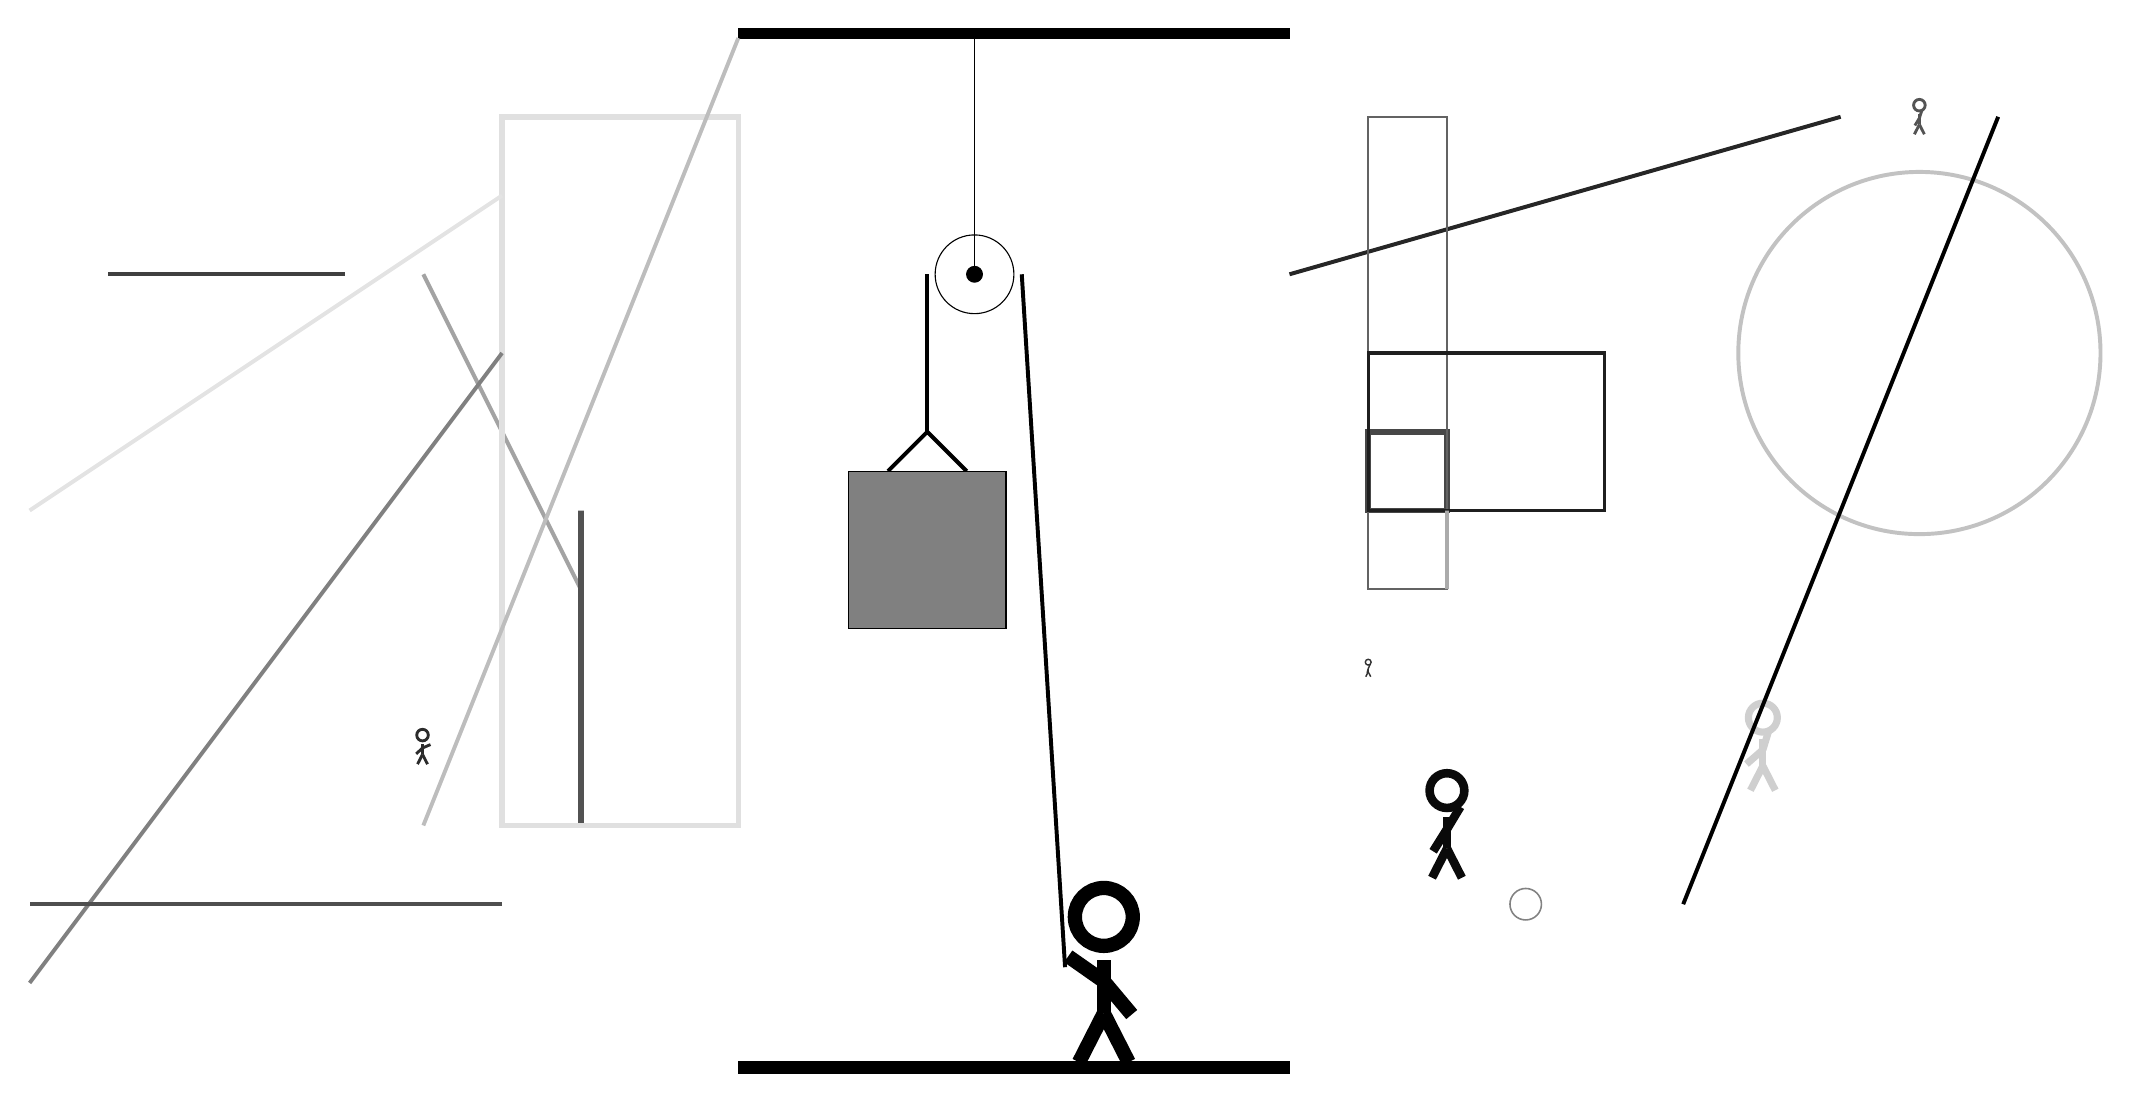
\begin{tikzpicture}
		%%%%% START %%%%%
		
		\draw[fill=black] (-2, 10) rectangle (5, 10.125);
		
		\draw (1, 7) circle (0.5);
		\draw[fill=black] (1, 7) circle (0.1);
		\draw (1, 10) -- (1, 7);
		
		\draw[line width=0.5mm] (-0.1, 4.5) -- (0.4, 5.0) -- (0.9, 4.5);
		\draw[fill=black!50] (-0.6, 4.5) rectangle (1.4, 2.5);
		
		\draw[line width=0.5mm, color=black!36](-4, 3) -- (-6, 7);
		
		\draw[line width=0.5mm, color=black!85](5, 7) -- (12, 9);
		\node[line width=0.7mm, color=black!19] at (11, 1) {\Strichmaxerl[5][41][73]};
		\node[line width=0.4mm, color=black!67] at (13, 9) {\Strichmaxerl[2][59][72]};
		\draw[line width=0.7mm, color=black!68] (-4, 0) rectangle (-4, 4);
		\draw[line width=0.7mm, color=black!12] (-2, 0) rectangle (-5, 9);
		
		\draw[line width=0.5mm, color=black!26](-2, 10) -- (-6, 0);
		
		\draw [line width=0.2mm, color=black!49](8, -1) circle (0.2);
		\node[line width=0.3mm, color=black!83] at (-6, 1) {\Strichmaxerl[2][43][23]};
		\draw[line width=0.7mm, color=black!72] (7, 4) rectangle (6, 5);
		
		\node[line width=0.5mm, color=black!80] at (6, 2) {\Strichmaxerl[1][75][65]};
		\draw[line width=0.3mm, color=black!61] (7, 3) rectangle (6, 9);
		\draw [line width=0.5mm, color=black!24](13, 6) circle (2.3);
		
		\draw[line width=0.4mm, color=black!88] (6, 4) rectangle (9, 6);
		\draw[line width=0.5mm, color=black!75](-7, 7) -- (-10, 7);
		\draw[line width=0.5mm, color=black!50](-5, 6) -- (-11, -2);
		
		\draw[line width=0.6mm, color=black!33] (7, 4) rectangle (7, 3);
		\node[line width=0.4mm, color=black!96] at (7, 0) {\Strichmaxerl[6][58][59]};
		\draw[line width=0.5mm, color=black!11](-5, 8) -- (-11, 4);
		\draw[line width=0.5mm, color=black!69](-5, -1) -- (-11, -1);
		\draw[line width=0.5mm, color=black!100](10, -1) -- (14, 9);
		
		\draw[line width=0.5mm] (0.4, 7) -- (0.4, 5.0);
		\centerarc[line width=0.5mm](1, 7)(0:180:0.6);
		\draw[line width=0.5mm](1.6, 7) -- (2.15, -1.8);
		
		\node at (2.6, -1.9) {\Strichmaxerl[10][-35][-50]};
		
		\draw[fill=black] (-2, -3) rectangle (5, -3.15);
		
		%%%%% END %%%%%
	\end{tikzpicture}
\end{document}